
编写CMake代码类似于用任何其他命令式语言编写代码:行从上到下、从左到右执行,偶尔会进入包含的文件或调用的函数。根据模式的不同(参见第1章),执行从源树的根文件(CMakeLists.txt)或者作为参数传递给CMake的.cmake脚本开始。

正如在前一章中所讨论,脚本支持大多数CMake语言(排除任何与项目相关的功能)。因此,它们是开始练习CMake语法的一个很好的方法,这就是在这里使用它们的原因。熟练地编写基本的列表文件之后,我们将在下一章准备实际的项目文件,可以使用以下命令运行脚本:

\begin{tcblisting}{commandshell={}}
cmake -P script.cmake
\end{tcblisting}

\begin{tcolorbox}[colback=blue!5!white,colframe=blue!75!black,title=Note]
CMake支持7位ASCII文本文件,以实现跨平台的可移植性。你可以同时使用\verb|\|n或\verb|\|r\verb|\|n作为换行符。3.0以上的CMake版本支持带有可选字节顺序标记(BOM)的UTF-8, 3.2以上的CMake版本支持UTF-16。
\end{tcolorbox}

CMake文件中的所有内容不是指令调用就是注释。

\subsubsubsection{2.2.1\hspace{0.2cm}注释}

像C++一样,有两种注释——单行注释和括号(多行)注释。但与C++不同的是,括号注释可以嵌套:

\begin{lstlisting}[style=styleCMake]	
# single-line comments start with a hash sign "#"
# they can be placed on an empty line
message("Hi"); # or after a command like here.

#[=[
bracket comment
	#[[
		nested bracket comment
	#]]
#]=]
\end{lstlisting}

多行注释的名称来自于它们的符号——以一个方括号([)、任意数量的等号(=)和另一个方括号[=[开始。要关闭一个括号注释,请使用相同数量的等号,并像这样反转括号:]=]。

使用\#在左括号标记前加上前缀是可选的,并且可以通过在括号注释的第一行添加另一个\#来快速禁用多行注释,就像这样:

\begin{lstlisting}[style=styleCMake]	
##[=[ this is a single-line comment now
no longer commented
	#[[
		still, a nested comment
	#]]
#]=] this is a single-line comment now
\end{lstlisting}

这是一个巧妙的技巧,但何时以及如何在CMake文件中使用注释呢?由于编写列表文件本质上是编程,因此将编码实践应用到文件中是一个好主意。遵循这种实践的代码通常认为是整洁的——这个术语由软件开发大师使用,如Robert C. Martin、Martin Fowler。什么是有益的,什么是有害的,经常会引起激烈的争论。同样,注释也在争论之中。

每件事都应该在个案的基础上进行判断,但通常的指导方针认为,好的注释至少提供以下其中之一:

\begin{itemize}
\item 
信息:可以解决诸如正则表达式模式或格式化字符串等复杂问题。

\item 
意图:当代码的意图在实现或接口中不明显时,可以解释代码的意图。

\item 
澄清:可以解释那些不容易重构或更改的概念。

\item 
结果警告:可以提供警告,特别是针对可能破坏其他内容的代码。

\item 
强调:可以强调难以用代码表达的想法的重要性。

\item 
法律条款:可以添加这个必要的法律条款,这通常不是程序员所擅长的领域。
\end{itemize}

如果可以的话,避免添加注释,并采用更好的命名实践,或者重构或修改代码。可以避免添加以下类型的注释:

\begin{itemize}
\item 
强制:强制添加这些注释是为了完整性,但不真正重要。

\item 
冗余:重复代码中已经明确写好的内容。

\item 
误导:若不跟随代码更改,则可能过时或不正确。

\item 
日志:记录更改的内容和时间(使用VCS代替)。

\item 
标记:仅用来进行标记。
\end{itemize}

编写没有注释的优雅代码非常困难,但它改善了读者的体验。因为我们花在读代码上的时间比写代码多,所以应该编写可读性好的代码,而不是仅仅试图快速地编写代码。建议查看本章末尾的扩展阅读部分,以获得一些关于干净代码的参考。若对注释特别感兴趣,可以找到我在YouTube上关于这个主题的视频链接。


\subsubsubsection{2.2.2\hspace{0.2cm}指令调用}

调用指令是CMake列表文件的基本功能。要执行指令,必须提供它的名称,后面跟着圆括号,在圆括号中可以包含一个以空格分隔的指令参数列表。

\begin{center}
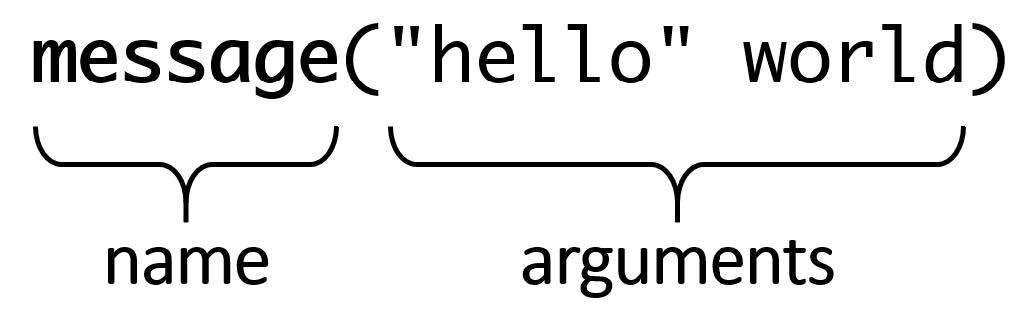
\includegraphics[width=0.3\textwidth]{content/1/chapter2/images/1.jpg}\\
图2.1 指令示例
\end{center}

命令名不区分大小写,但在CMake社区中有一个约定,即在指令名中使用snake\_case(即小写单词与下划线连接)。

也可以定义自己的命令,我们将在“控制结构"一节中介绍这些指令。

与C++相比,CMake中的指令调用不是表达式。不能为调用指令提供另一个指令作为参数,因为括号之间的所有内容都会解释为该指令的参数。

CMake指令不需要在调用结束时使用分号。这可能是因为每行源代码最多可以包含一个命令调用,后面跟着一个可选的单行注释。或者,整行必须是括号注释的一部分。所以,这些是唯一允许的格式:

\begin{lstlisting}[style=styleCMake]	
command(argument1 "argument2" argument3) # comment
[[ multiline comment ]]
\end{lstlisting}

不允许将指令放在括号注释后面:

\begin{lstlisting}[style=styleCMake]	
[[ bracket
]] command()
\end{lstlisting}

删除所有注释、空格和空行之后,得到一个指令列表。CMake语法真的很简单,但这是一件好事吗?我们怎么处理变量呢?或者,如何指导执行的流程?

CMake为这些操作提供了命令和更多的功能。为了使事情更简单,将在介绍不同示例时介绍相关指令,它们可以分为三类:

\begin{itemize}
\item 
脚本指令:脚本指令总是可用的,会改变指令处理器、访问变量的状态,并影响其他指令和环境。

\item 
项目指令:这些指令在项目中可用,操纵项目状态并构建目标。

\item 
CTest指令:这些指令在CTest脚本中可用,管理测试。
\end{itemize}

我们将在本章中介绍脚本指令(因为它们在项目中也很有用)。项目和CTest指令将在接下来的章节中讨论,我们将介绍与构建目标(第3章)和测试框架(第8章)相关的概念。

实际上,每个指令都依赖于该语言的其他元素来发挥作用:变量、条件语句,以及最重要的指令参数。让我们看看如何使用这些参数。

\subsubsubsection{2.2.3\hspace{0.2cm}指令参数}

许多指令需要用空格分隔的参数来参数化它们的行为。正如在图2.1中看到的,参数周围的引号发生了一些奇怪的事情。有些论点有引用,有些没有,这是怎么回事?

在底层,CMake识别的唯一数据类型是字符串。这就是为什么每个命令的参数都期望0个或多个字符串。但是普通的静态字符串并不是很有用,特别是不能嵌套指令调用时。这就是参数发挥作用的地方——CMake将计算静态字符串的每个参数,然后将它们传递到命令中。求值意味着字符串插值,或者用另一个值替换字符串的部分。这可能意味着替换转义序列、扩展变量引用(也称为变量插值)和解包列表。

根据上下文的不同,可以根据需要启用这种计算。因此,CMake提供了三种类型的参数:

\begin{itemize}
\item 
方括号参数

\item 
引号参数

\item 
非引号参数
\end{itemize}

每种参数类型提供不同的求值级别,并有一些小特点。

\hspace*{\fill} \\ %插入空行
\noindent
\textbf{方括号参数}

方括号参数不会进行求值,并用于将多行字符串作为单个参数逐字传递给命令。所以将包括制表符和换行符形式的空白。

这些参数的结构与注释完全相同——以[=[开始,以]=]结束,其中开始和结束标记中的等号数量必须匹配(跳过等号也可以,但必须匹配)。与注释的唯一区别是不能嵌套括号参数。

下面是message()指令使用这种参数的示例,将所有传递的参数打印到屏幕上:

\begin{lstlisting}[style=styleCMake]
# chapter02/01-arguments/bracket.cmake	

message([[multiline
bracket
argument
]])

message([==[
	because we used two equal-signs "=="
	following is still a single argument:
	{ "petsArray" = [["mouse","cat"],["dog"]] }
]==])
\end{lstlisting}

上面的例子中,可以看到不同形式的括号参数。第一个跳过了等号,将结束标记放在单独的行上,在输出中显示为空行:

\begin{tcblisting}{commandshell={}}
$ cmake -P chapter02/01-arguments/bracket.cmake
multiline
bracket
argument

  because we used two equal-signs "=="
  following is still a single argument:
  { "petsArray" = [["mouse","cat"],["dog"]] }
\end{tcblisting}

第二种形式在传递包含双括号(]])(在代码片段中突出显示)的文本时很有用,不会解释为标记参数的结束。

这类括号参数的用途有限——通常用于包含较长的文本块。大多数情况下,需要一些更动态的东西,比如引用参数。

\hspace*{\fill} \\ %插入空行
\noindent
\textbf{引号参数}

带引号的参数类似于常规的C++字符串——这些参数将多个字符组合在一起,包括空格,它们将展开转义序列。与C++字符串一样,它们的开始和结束都使用双引号("),因此要在输出字符串中包含一个引号字符,必须使用反斜杠对其进行转义(\verb|\|")。

也支持其他转义序列: \verb|\|\verb|\|表示字面反斜杠,\verb|\|t是一个制表符,\verb|\|n 是换行符,和\verb|\|r是一个回车符。

这就是与C++字符串的相似之处。带引号的参数可以跨越多行,将插入变量引用。可以把它们想象成拥有来自C语言的内置sprintf函数,或者C++20的std::format函数。要将变量引用插入到参数中,可以将变量名包装在字符串中,就像这样:\$\{name\}。

我们将在“变量”一节中更多地讨论变量引号。

\begin{lstlisting}[style=styleCMake]
# chapter02/01-arguments/quoted.cmake
	
message("1. escape sequence: \" \n in a quoted argument")
message("2. multi...
	line")
message("3. and a variable reference: ${CMAKE_VERSION}")
\end{lstlisting}

能猜到前面脚本的输出中有多少行吗?

\begin{tcblisting}{commandshell={}}
$ cmake -P chapter02/01-arguments/quoted.cmake
1. escape sequence: "
 in a quoted argument
2. multi...
line
3. and a variable reference: 3.16.3
\end{tcblisting}

没错——我们有一个转义引号字符、一个转义换行符和一个字面换行符。所有这些都将打印在输出中。我们还访问了一个内置的CMAKE\_VERSION变量,可以看到在最后一行正确插入了该变量。

\hspace*{\fill} \\ %插入空行
\noindent
\textbf{非引号参数}

最后一种类型的参数在编程世界中肯定有点罕见。我们已经习惯了字符串必须以这样或那样的方式分隔的事实,例如:单引号、双引号或反斜杠。CMake背离了这一惯例,引入了不加引号的实参。我们可能会说,删除分隔符使代码更容易阅读,就像跳过分号一样。这是真的吗?

不加引号的实参计算转义序列和变量引用。但是,要小心使用分号(;),就像在CMake中一样,其会当作分隔符对待。CMake会将包含它的参数拆分为多个参数。若需要使用,可以使用反斜杠对其进行转义(\verb|\|;)。这就是CMake管理列表的方式。

可能会发现这些参数是最复杂的,所以这里有一个例子可以来表明这些参数是如何划分的:

\begin{center}
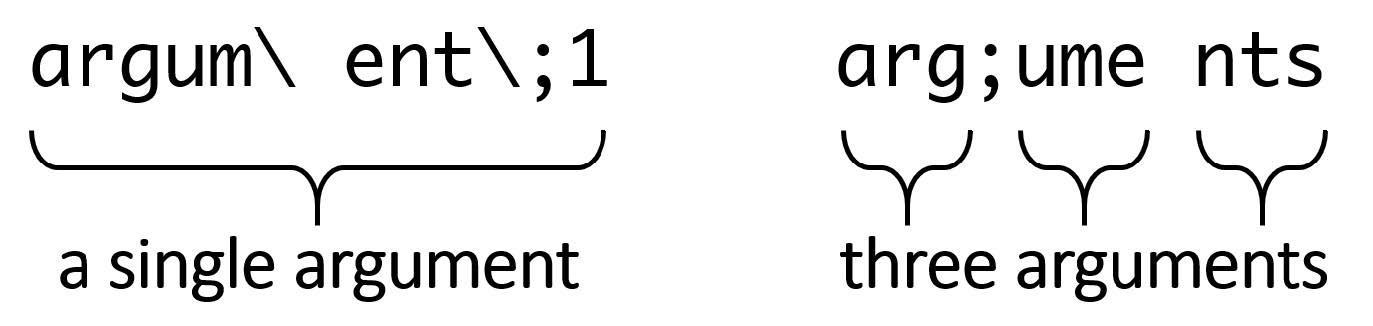
\includegraphics[width=0.5\textwidth]{content/1/chapter2/images/2.jpg}\\
图2.2 转义字符将使后续的字符解释为单个参数
\end{center}

\begin{tcolorbox}[colback=black!5!white,colframe=black!75!black,title=问题]
为什么“一个值是作为一个参数传递,还是作为多个参数传递”很重要?一些CMake指令需要特定数量的参数,并忽略任何开销。若参数分离,就会出现难以调试的错误。
\end{tcolorbox}

不加引号的参数不能包含未转义的引号(")、井号(\#)和反斜杠(\verb|\|)。若不够用,只有当它们形成正确的、匹配的对时才允许使用括号(())。也就是说,将从一个左括号开始,然后在关闭指令参数列表之前关闭它。

来看看以上规则的例子:

\begin{lstlisting}[style=styleCMake]
# chapter02/01-arguments/unquoted.cmake
	
message(a\ single\ argument)
message(two arguments)
message(three;separated;arguments)
message(${CMAKE_VERSION}) # a variable reference
message(()()()) # matching parentheses
\end{lstlisting}

上面的输出是什么?让我们来看看:

\begin{tcblisting}{commandshell={}}
$ cmake -P chapter02/01-arguments/unquoted.cmake
a single argument
twoarguments
threeseparatedarguments
3.16.3
()()()
\end{tcblisting}

即使是像message()这样的简单命令,也非常讲究参数之间不加引号的分隔:

\begin{itemize}
\item 
显式转义单个参数中的空格时,将正确打印空格。

\item 
因为message()不会添加任何空格,所以两个参数和三个单独的参数会粘在一起。
\end{itemize}

既然已经了解了如何处理CMake参数的复杂性和特殊之处,就可以学习下一个有趣的主题了——使用各种变量。









